\subsubsection{Kalman Filter}
%\scriptsize
\textbf{Grundgedanke} Beim Kalman Filter wird der Kalman Gain nach dem
kleinsten Fehlerquadrat gesch�tzt. Speziell am Kalman ist, dass Messgr�ssen
mithilfe der Zustandsgr�ssen und einem Rauschsignal definiert ist. \\
\textbf{Voraussetzungen}
\begin{aufzaehlung}
   	\item Physikalisches Modell/Systementwicklung (f�r normales sogar ein
   	lineares Modell)
   	\item Messwerte, auch eine Sensorfusion m�glich (mehrere Messwerte f�r ein
   	Systemzustand)
   	\item f�r normales Kalman: linearer Zusammenhang zwischen Messwerten und
   	Zustandsgr�ssen
\end{aufzaehlung}
\begin{minipage}{8cm}
	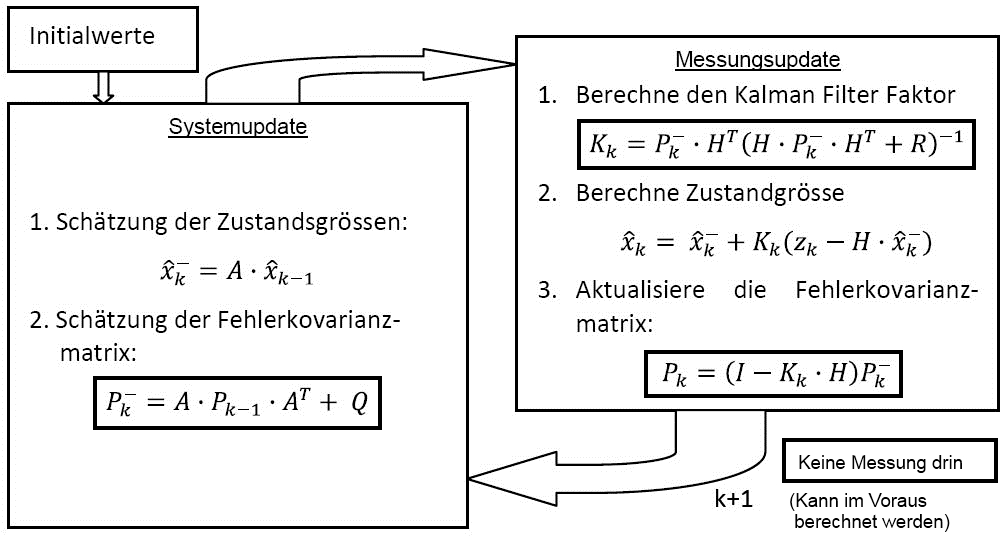
\includegraphics[width=8cm]{Content/AdaptSigVer/KalmanFilter.jpg}
	
	\begin{itemize}
		\item $\hat{x}_{k-1}$ und $P_{k-1}$ ben�tigen Initialisierungswerte
		\item $P_K$ und $K_K$ k�nnen offline vorausberechnet werden, wenn das System nicht �ndert
	\end{itemize}
	
\end{minipage}
\begin{minipage}{11cm}
	\small
	\textbf{Funktion}
		\begin{liste}
	    	\item A Systementwicklungsmatrize: Physikalische Modell
	    	\item K Kalman Gain: Gewichtet interne Sch�tzung und die Messungen der
	    	einzelnen Sensoren (0=Nur interne Sch�tzung;1=nur Messung)
	    	\item H Messmatrize: Zusammenhang zwischen Mess- und Zustandsgr�ssen
	    	\item P (Fehlerkovarianzma.) Sch�tzgr�sse f�r den Fehler. Je gr�sser desto
	    	mehr wird aktuelle Messung ber�cksichtigt. Beim normalen Kalman Filter
	    	konvergiert dieser mit der Zeit.
	    	\item z: Messwerte (auch von mehreren gleichartigen Sensoren m�glich)
	    	\item x: Zustandsgr�ssen
	    	\item Initialwert: Systemwerte beliebig; Fehlerkovarianzmatrize sehr
	    	gross w�hlen, so dass zuerst nur die Messung ber�cksichtigt wird
	    	\item Q Standartabweichung System (Systemrauschen)
	    	\item R Standartabweichung der Sensoren (Messrauschen)
				\item Das Verh�ltniss von Q zu R ist f�r die Filtereinstellung verantwortlich.\newline
				$\frac QR$ gross $\rightarrow$ vertraut mehr den Messdaten\newline \hspace{4cm} $\frac QR$ klein $\rightarrow$ vertraut mehr den Systemeigenschaften
	    \end{liste}
	\normalsize
\end{minipage}\\
\\
\textbf{Vereinfachtes Prinzip des Kalman-Filters}\\
\begin{minipage}{14.5cm}
Man hat zwei ungenaue Sensoren $T_1$ und $T_2$, welche das gleiche Signal messen und deren Standartabweichungen $\sigma_1$ und $\sigma_2$ bekannt sind. Der beste
Sch�tzer $\hat{T}$ wird wie folgt errechnet:\\
\end{minipage}
\hspace{0.25cm}
\begin{minipage}{5cm}
$\hat{T}=\frac{\sigma_1^2}{\sigma_1^2+\sigma_2^2}\cdot T_2+\frac{\sigma_2^2}{\sigma_1^2+\sigma_2^2}\cdot T_1$
\end{minipage}